% 2019-01-30

\documentclass[10pt]{article}
\usepackage[T1]{fontenc}
\usepackage{amssymb}
\usepackage{amsmath}
\usepackage{graphicx}
% \begin{figure}[h]
% \centering
% \includegraphics[width=6.5in]{folder/photo.png}
% \caption{}
% \label{}
% \end{figure}



\usepackage{tikz}
\usetikzlibrary{arrows}
\usepackage{subfigure}
\usepackage{stackrel}
\usepackage{blindtext}

\usepackage[url=false]{biblatex}
\addbibresource{library.bib}

\oddsidemargin=0.15in
\evensidemargin=0.15in
\topmargin=-.5in
\textheight=9in
\textwidth=6.25in

\usepackage[colorlinks=true,breaklinks,pdfpagemode=none,linkcolor=blue,citecolor=blue]{hyperref}

\usepackage{enumerate}
% \vspace{-6pt}
% \begin{itemize}
%     \setlength{\itemsep}{0pt}%
%     \setlength{\parskip}{0pt}%
%     \item Item 1
%     \item Item 2
%         \begin{itemize}
%             \setlength{\itemsep}{0pt}%
%             \setlength{\parskip}{0pt}%
%             \item Sublist Item 1
%             \item Sublist Item 2
%         \end{itemize}
%         \item Item 3
% \end{itemize}
% \vspace{-6pt}


\usepackage{enumitem}
\setlist{itemsep=0mm}

\usepackage{amsmath,amsfonts,amssymb,bm}


\begin{document}

   \noindent
   \begin{center}

   \hrulefill
   
   \vspace{5pt}
   
   \makebox[\textwidth]{ {\bf Energy Systems Analysis} \hfill  A.D. Smith 2019}
   \vspace{0pt}
   
   {\Large \hfill  Lecture 9. BEM: Climate Zones, Commercial and Residential Buildings}
   \vspace{5pt}
   
  
   \hrulefill
   \end{center}

   {\color{darkgray}{{\center{ \small{      ``Discussions of sun, air, and water resources available on a site are influenced both by the `private' needs of a building and the `public' patterns of resource availability, which should remain accessible to all.''
\\%[3pt]
\rightline{{\rm --- Grondzik and Kwok \cite{Grondzik2014-gt}}}}}}}}

\section{Climate}

\begin{quote}
\textbf{Climate} is a long-term statistically derived picture of weather. \textbf{Weather} is what happened today or yesterday, while climate has historically been a picture of what happened over the past 10, 15, or 20 years. \cite{Grondzik2014-gt}
\end{quote}

The climate where buildings and distributed energy resources are located will determine the external conditions they experience during their lifetime, and thus influence how they perform. Architects and engineers need an understanding of the climate that will influence a particular site to make good design decisions for a building (e.g. selecting the proper size air conditioning unit, choosing insulation and vapor barriers for walls, or placing windows and shading on the building). Engineers, designers, and operators also need to evaluate the ``sun, air, and water resources available'' to make good decisions about whether and how to select distributed generation and storage or to implement demand-side energy measures, which we'll discuss later with distributed energy resources.

Modelers need to have weather data that represents the climate that is expected, a need usually served by the TMY files mentioned in Lecture 8. If a particular year's weather is of interest (or relevant to a calibration effort), then the modeler needs an AMY file as mentioned in Lecture 8. There are existing research efforts to provide future weather year files \cite{C_Bianchi_DL_Mendoza_RC_Didier_TD_Tran_AD_Smith2017-uk}, incorporating projections for climate change, but these are rarely used in practice.

\subsection{Microclimate}

\begin{quote}
    Local variations constitute microclimates, which have some characteristics distinctly different from the conditions prevailing in the larger macroclimate. The characteristics of a microclimate are influenced by the interaction of the site conditions with the macroclimate. \cite{Grondzik2014-gt}
\end{quote}

The \textbf{microclimate} represents the 'local' weather for a restricted local area, which could be as small as an area at the corner of an external wall (where changing airflow patterns will affect the observed meteorology). It is highly related to the surrounding climate, but unique conditions can affect the temperature, humidity, wind speed, radiation, and other weather-related variables, such as:

\begin{itemize}
    \setlength{\itemsep}{0pt}%
    \setlength{\parskip}{0pt}%
    \item Presence of walls, windows, and overhangs
    \item Human interaction with the building or landscape
    \item Presence of concrete, asphalt, or different types of ground cover
    \item Changes in ground cover or other surface characteristics
    \item Presence of other buildings or structures
\end{itemize}

\subsection{Urban Heat Island}

\begin{quote}
    The most obvious reason for a city's relative year-around warmth is its concentration of heat sources: the air conditioner condensers, furnaces, electric lighting in buildings, and internal combustion engines in cars. \ldots It appears that cities and industrial regions of the world release less internal heat per capita as people live and work closer together---although the heat density (temperature) is greater. \cite{Grondzik2014-gt}
\end{quote}

The term \textbf{urban heat island (UHI) effect}  is a recognition of the observed data showing that temperatures in urban areas are higher than surrounding suburban or rural areas, even if the larger climate and meteorology they experience is similar. This is due to more concentration among heat sources, and less opportunity to reject heat away from the built environment \cite{Grondzik2014-gt}.

\section{Climate Zones}

\begin{quote}
    Our most familiar names for climates describe their most severe season \ldots This is a convenient means of description, but it can be misleading for designers. ``Cold'' climates can have very hot, sometimes humid, summer days; hot-arid climates can have bitterly cold winter conditions. Before designing buildings that will interact with exterior conditions to provide indoor comfort, we should know in some detail the character of those conditions. \cite{Grondzik2014-gt}
\end{quote}

Because both dry bulb temperature and moisture are important or building design and performance, these are the key features used to classify a \textbf{climate zone}, an identified geographic region that experiences similar climate patterns. At its most detailed, we divide the contiguous United States into 7 climate zones, Figure \ref{CZs}, and assessments are made county by county. Alaska has an additional Climate Zone 8, which is extremely cold. There is also a Climate Zone 0, which is extremely hot, existing near the equator but not within the U.S.  You may also see these referred to as `climate regions' or `ANSI/ASHRAE/IESNA climate zones' as they are part of standards published by these organizations. For more about the technical meaning and determination of climate zones, see the DOE's Climate Zones page \cite{noauthor_undated-ax}. 

            \begin{figure}[h]
            \centering
            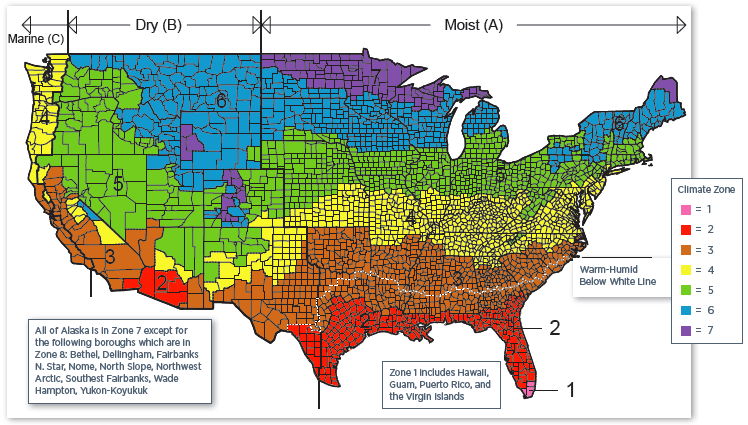
\includegraphics[width=6.5in]{extras09/climatezones.png}
            \caption{International Energy Conservation Code (IECC) Climate Zones in the Lower 48 States \cite{Baechler2015-me}}
            \label{CZs}
            \end{figure}


Living in Utah near the mountain ranges, you can probably think of a place where more than one climate zone exists within the same county. For example, Alta is located within Salt Lake County, yet you might have had the experience of visiting Alta and seeing notably lower temperatures, or seeing snow falling at Alta while rain falls on Salt Lake City. So even though Alta falls within the Climate Zone 5 region on the map, a thoughtful engineer might choose to follow design criteria that are targeted at Zone 6 instead.

\section{Commercial Buildings}

For building energy modeling purposes, the DOE provides a set of example building models called the \textbf{Commercial Prototype Building Models}:
\url{https://www.energycodes.gov/development/commercial/prototype_models}. These are based on the CBECS survey mentioned in Lecture 3. You may also come across the precursors to the Commercial Prototype Buildings, called the Commercial Reference Buildings \cite{noauthor_undated-hj}.

They are designed for different code years of ANSI/ASHRAE/IES Standard 90.1, ``Energy Standard for Buildings Except Low-Rise Residential Buildings'' \cite{ashrae90.1}, which is often adopted and incorporated into formal building codes. The DOE has a reference page on \url{www.energycodes.gov} where you can learn more about building codes \cite{noauthor_undated-dt}.

The main designations for building types within this sector are:
\begin{itemize}
    \setlength{\itemsep}{0pt}%
    \setlength{\parskip}{0pt}%
    \item Small Office
    \item Medium Office
    \item Large Office
    \item Stand-alone Retail
    \item Strip Mall
    \item Primary School
    \item Secondary School
    \item Outpatient Healthcare
    \item Hospital
    \item Small Hotel
    \item Large Hotel
    \item Warehouse
    \item Quick Service Restaurant
    \item Full Service Restaurant
    \item Mid-rise Apartment
    \item High-rise Apartment
\end{itemize}

We will use them when we need examples of commercial buildings to use in our modeling work.

\section{Residential Buildings}

For building energy modeling purposes, the DOE provides a set of example building models called the Residential Prototype Building Models:  \url{https://www.energycodes.gov/development/residential/iecc_models}. These are based on the RECS survey mentioned in Lecture 3. They are designed for different code years of the International Energy Conservation Code (IECC) {\color{blue}\cite{IECCresources}}.

There are only two major designations for residential prototype models:
\begin{itemize}
    \setlength{\itemsep}{0pt}%
    \setlength{\parskip}{0pt}%
    \item Single-family detached house
    \item Multi-family low-rise apartment building\\(Remember that mid- and high-rise apartments are classified with commercial buildings).
\end{itemize}

If you download the residential files available for Utah, you will see that in addition to the code year, you have a few more options to choose from:

\begin{itemize}
    \setlength{\itemsep}{0pt}%
    \setlength{\parskip}{0pt}%
    \item Gas furnace, oil furnace, electric heat or heat pump
    \item Crawlspace, slab, heated basement or unheated basement
\end{itemize}

We will use them as a starting point when we need examples of residences to use in our modeling work.


% license
\bigskip

\noindent
\texttt{\footnotesize RESTRICTED PUBLIC LICENSE --- READ BEFORE SHARING. This is a draft version made available by Amanda D. Smith under a Creative Commons Attribution-NonCommercial-ShareAlike license. 
\href{https://creativecommons.org/licenses/by-nc-sa/4.0/}{CC BY-NC-SA 4.0}}

% references
\newpage
\printbibliography

\end{document}